%al posto di template.tex va messo il nome del file del livello superiore
\documentclass[../PianoProgetto.tex]{subfiles}

\begin{document}
%al posto di nome sezione va messo il nome della sezione appunto
\section{Pianificazione}

	Di seguito saranno elencate le durate e le caratteristiche di ogni fase. I tempi sono stati pensati per permettere uno slack sufficiente, in modo da mitigare i rischi relativi alle tempistiche.
	
	\subsection{Fase A: Analisi}
	
	\textbf{Periodo: dal 2015-11-23 al 2016-01-22}

	Questa fase comincia con la presentazione in aula delle regole del progetto didattico e termina con la scadenza della consegna della Revisione dei Requisiti.

	Le sottofasi sono le seguenti:
	\begin{enumerate}
		\item Individuazione strumenti: Verranno scelti gli strumenti che saranno utilizzati per la stesura dei documenti, per il supporto e per il tracciamento dei requisiti;
		\item Norme Di Progetto: Dopo aver individuato gli strumenti si potrà procedere alla stesura del documento \textit{"Norme di Progetto v1.00"}. Questo documento sarà utilizzato indipendentemente dal capitolato che sarà preso in appalto;
		\item Stesura documentazione: In questa fase conosciamo gli strumenti da utilizzare e le norme per scrivere un documento, quindi possiamo iniziare la stesura di:
		\begin{itemize}
		\item Studio Di Fattibilità: Vengono valutati pro e contro di tutti i capitolati proposti e viene redatto il documento \textit{"Studio di Fattibilità v1.00"}. Viene quindi scelto il capitolato da sviluppare;
		\item Analisi Dei Requisiti: Viene steso il documento \textit{"Analisi dei Requisiti v1.00"}. Prima e durante la stesura di questo documento verranno organizzati degli incontri con il proponente per consolidare i requisiti stesi o per chiarire le idee sui requisiti da stendere;
		\item Piano Di Progetto: Si stende il documento \textit{"Piano di Progetto v1.00"} per regolare le attività che il team dovrà svolgere;
		\item Piano Di Qualifica: Si redige il documento \textit{"Piano di Qualifica v1.00"};
		\item Glossario: viene incrementato il file \textbf{"Glossario.xml"} e steso in modo automatico il documento \textit{"Glossario v1.00"}.
		\end{itemize}
	\end{enumerate}
		
		\subsubsection{Diagramma di Gantt – Fase A}
			\begin{figure}[!h]
				\centering
				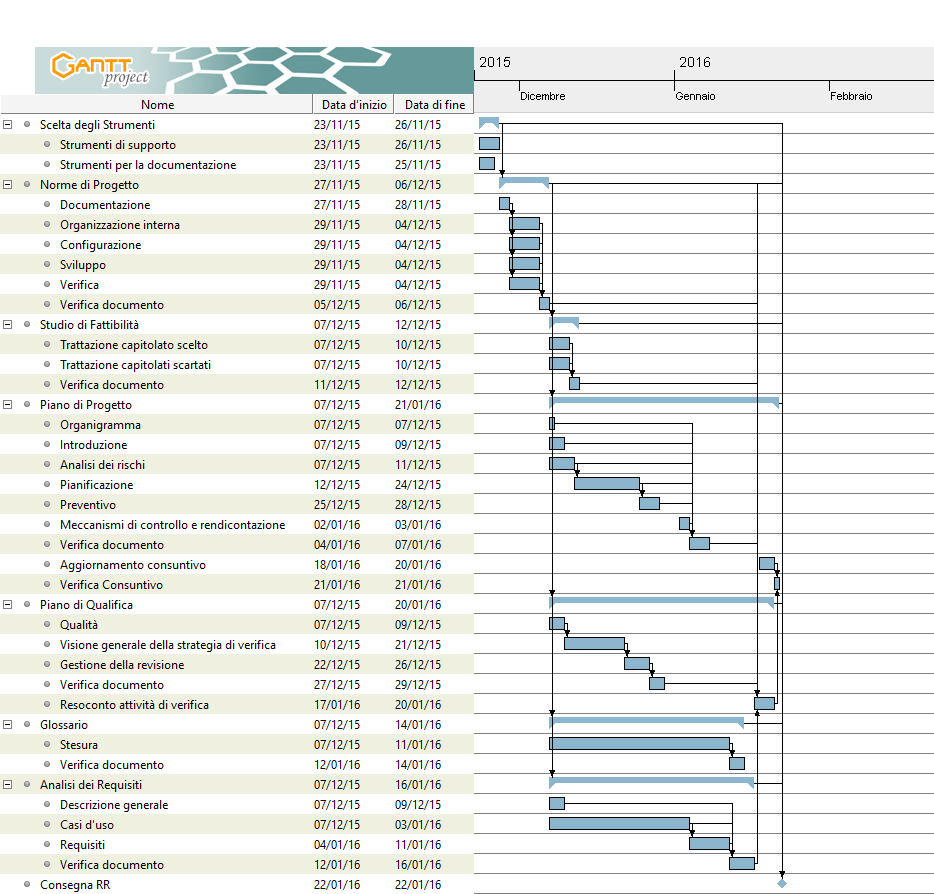
\includegraphics[width=\textwidth]{gantt_png/1-analisi}
				\caption{Gantt - Fase A}
				\label{fig:Gantt - Fase A}
			\end{figure}			
	
	\subsection{Fase AD: Analisi di Dettaglio}
		\textbf{Periodo: dal 2016-02-16 al 2016-02-22}

				Questa fase comincia al termine della Fase A. È caratterizzata da una nuova analisi di tutti i documenti redatti nella fase precedente e dalla correzione in base alle richieste e segnalazioni del committente. Gli analisti provvedono all’individuazione di nuovi requisiti, alla correzione dei requisiti segnalati e si provvede all’incremento di tutti gli altri documenti.  Aggiornati i requisiti, si terrà un incontro con il proponente per la loro verifica.
					
		\subsubsection{Diagramma di Gantt – Fase AD}
			\begin{figure}[!h]
				\centering
				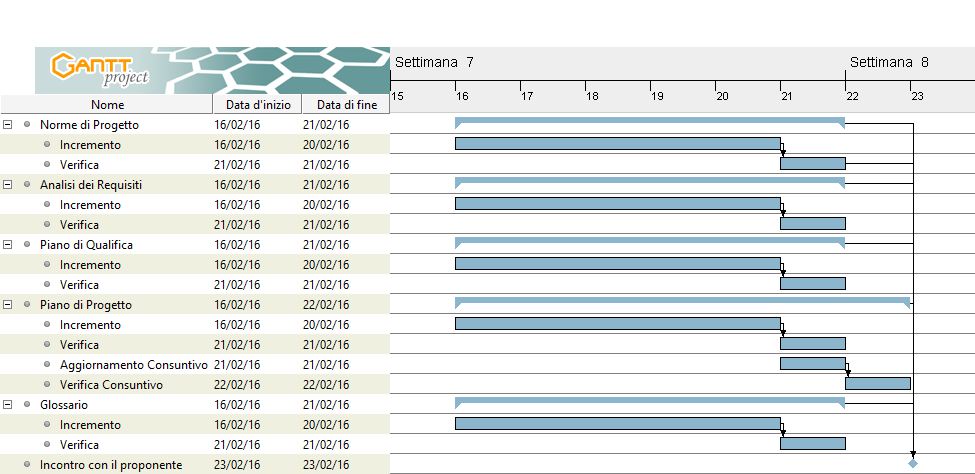
\includegraphics[width=\textwidth]{gantt_png/2-analisi_di_dettaglio}
				\caption{Gantt - Fase AD}
				\label{fig:Gantt - Fase AD}
			\end{figure}

	\subsection{Fase PA: Progettazione Architetturale}
		\textbf{Periodo: dal 2016-02-23 al 2016-03-18}
		
		Questa fase comincia con la fine della Fase AD e termina con l’incontro con il Proponente per mostrare l’architettura scelta. Le attività di questa fase sono:
		\begin{itemize}
			\item Norme di Progetto: Viene fatto un incremento alle norme per poter stendere il documento \textit{“Specifica Tecnica”}. Viene successivamente fatta una verifica per fissare una baseline al documento che diventerà \textit{“Norme di Progetto v3.00”};

			\item Specifica Tecnica: Questa attività caratterizza la Progettazione Architetturale. Il \progettista\ stende la \textit{“Specifica Tecnica”} che contiene le scelte progettuali, ad alto livello, che il progetto dovrà avere. Saranno quindi descritti quali design pattern implementerà, l’architettura logica del software, i principali flussi di controllo e il tracciamento dei requisiti;

			\item Glossario: Viene fatto un incremento al \glossario aggiungendo tutti i vocaboli che si ritiene importante siano inclusi. Viene successivamente fatta una verifica per fissare una baseline al documento che diventerà \textit{“Glossario v3.00”};

 			\item Piano di Qualifica: l’incremento consiste nell’aggiungere al documento \pianodiqualifica il dettaglio dell’esito della Revisione dei Requisiti e la parte della pianificazione dei test. Questa attività genererà, dopo una verifica e validazione, il file \textit{“Piano di Qualifica v3.00”};

			\item Piano di Progetto: l’incremento che sarà fatto al documento \pianodiprogetto in questa fase consiste nell’apportare correzioni nella divisione delle attività e stillare il consuntivo di questo periodo. Dopo un’accurata verifica che fisserà una nuova baseline e la validazione il documento diventerà \textit{“Piano di Progetto v3.00”}.
		\end{itemize}
		
		\subsubsection{Diagramma di Gantt – PA}
			\begin{figure}[!h]
				\centering
				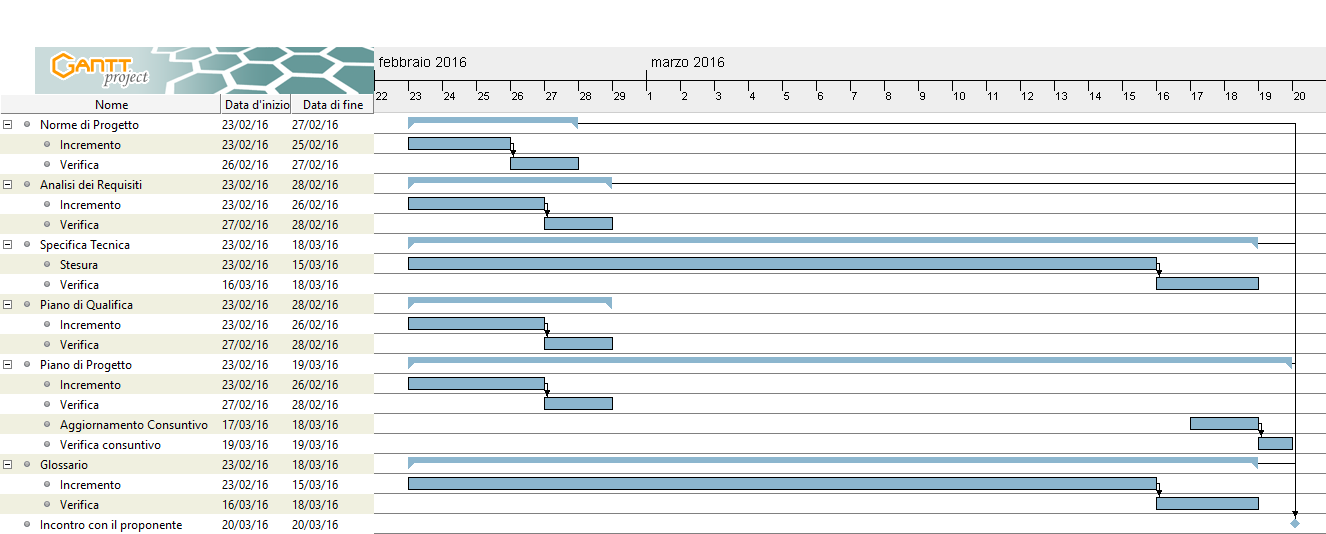
\includegraphics[width=\textwidth]{gantt_png/3-progettazione_architetturale}
				\caption{Gantt - Fase PA}
				\label{fig:Gantt - Fase PA}
			\end{figure}
			
	\subsection{Fase PDROB: Progettazione di Dettaglio e codifica dei Requisiti Obbligatori}
		\textbf{Periodo: dal 2016-03-19 al 2016-04-18}
		
		Questa fase comincia con la fine della Fase PA e termina con la consegna della Revisione di Progetto. Le attività di questa fase saranno le seguenti:
		\begin{itemize}
			\item Definizione di Prodotto: viene steso il documento \textit{“Definizione di Prodotto v1.00”}. Esso definisce la struttura interna del sistema e le relazioni dei componenti del prodotto relativi ai requisiti obbligatori.

			\item Codifica: con quest’attività inizia lo sviluppo da parte dei programmatori dei requisiti obbligatori. Sarà dunque seguito quanto riportato nel documento \textit{“Definizione di Prodotto v1.00”};

			\item Esecuzione test: verranno eseguiti automaticamente tutti i test di unità previsti dal documento \textit{“Piano di Qualifica v 4.00”};

			\item Manuale Utente e Manuale Amministratore: comincia la stesura dei manuali che forniranno indicazioni agli utilizzatori del sistema.

			\item Incremento e Verifica Documenti: vengono eseguite modifiche ai documenti già scritti, se necessario.

			\item Glossario: vengono aggiunti al file \textbf{“Glossario.xml”} i vocaboli dei quali si ritiene necessaria una definizione formale. Alla fine di questa fase vieni quindi generato il documento \textit{“Glossario v4.00”}.
		\end{itemize}

		\subsubsection{Diagramma di Gantt – PDROB}
			\begin{figure}[!h]
				\centering
				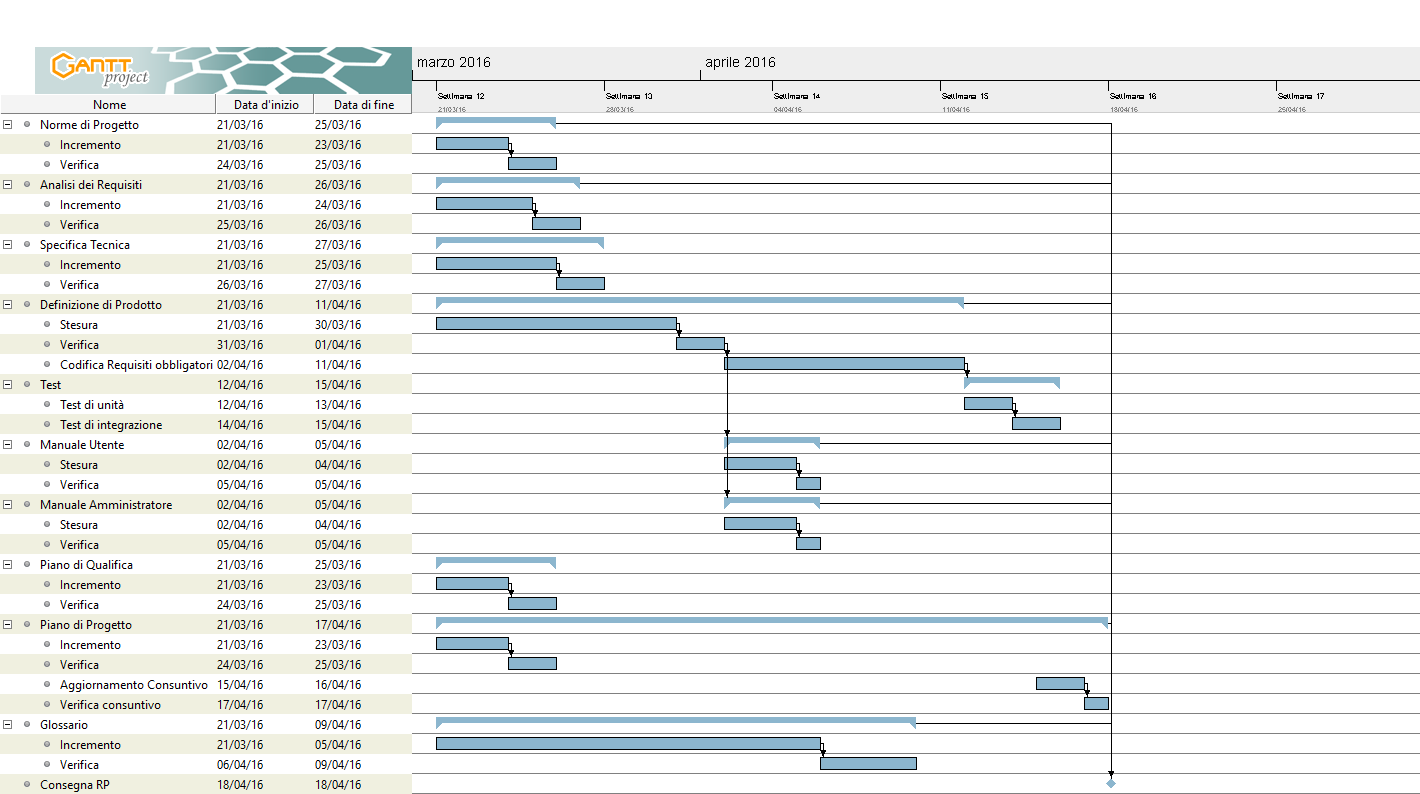
\includegraphics[width=\textwidth]{gantt_png/4-requisiti_obbligatori}
				\caption{Gantt - Fase PDROB}
				\label{fig:Gantt - Fase PDROB}
			\end{figure}

	\subsection{Fase PDRD: Progettazione di Dettaglio e codifica dei Requisiti Desiderabili}
		\textbf{Periodo: dal 2016-04-19 al 2016-05-09}
		
		Questa fase comincia con la fine della Revisione di Progetto e termina l’incontro con il proponente al fine di mostrare il prototipo con i requisiti obbligatori e desiderabili. Le attività di questa fase saranno le seguenti:

		\begin{itemize}
			\item Definizione di Prodotto: Viene steso il documento \textit{“Definizione di Prodotto v2.00”}. Esso definisce la struttura interna del sistema e le relazioni dei componenti del prodotto relativi ai requisiti desiderabili.

			\item Codifica: Con quest’attività inizia lo sviluppo da parte dei programmatori dei requisiti desiderabili. Sarà dunque seguito quanto riportato nel documento \textit{“Definizione di Prodotto v2.00”};

	 		\item Esecuzione test: verranno eseguiti automaticamente tutti i test di unità e integrazione previsti dal documento \textit{“Piano di Qualifica v 5.00”};

			\item Manuale Utente e Manuale Amministratore: Comincia la stesura dei manuali che forniranno indicazioni agli utilizzatori del sistema.

			\item Incremento e Verifica Documenti: Vengono eseguite modifiche ai documenti già scritti, se necessario.

			\item Glossario: Vengono aggiunti al file \textbf{“Glossario.xml”} i vocaboli dei quali si ritiene necessaria una definizione formale. Alla fine di questa fase vieni quindi generato il documento \textit{“Glossario v5.00”}.
		\end{itemize}
		
		\subsubsection{Diagramma di Gantt – Fase PDRD}
			\begin{figure}[!h]
				\centering
				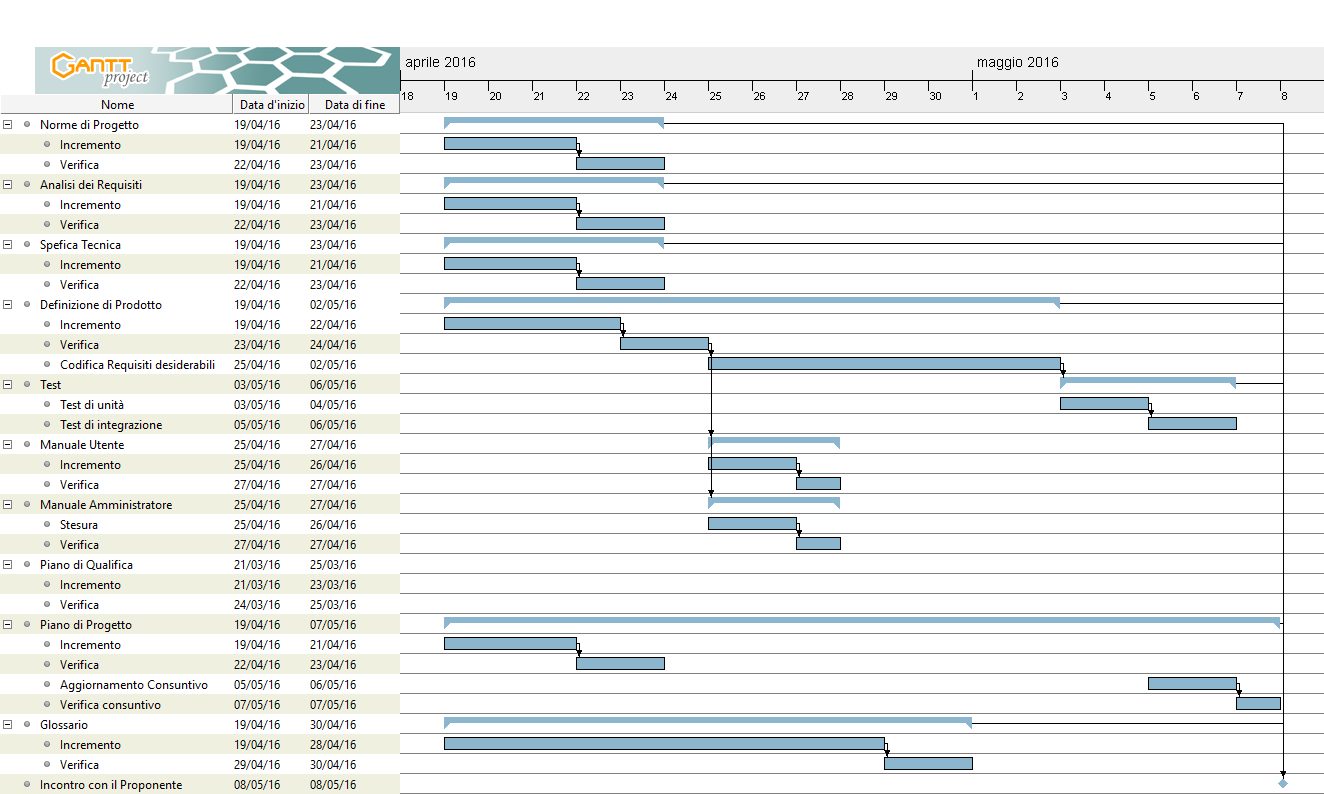
\includegraphics[width=\textwidth]{gantt_png/5-requisiti_desiderabili}
				\caption{Gantt - Fase PDRD}
				\label{fig:Gantt - Fase PDRD}
			\end{figure}
			

	\subsection{Fase PDROP: Progettazione di Dettaglio e codifica dei Requisiti Opzionali}
		\textbf{Periodo: dal 2016-05-10 al 2016-05-23}
		
		Questa fase comincia dopo la visione da parte del proponente del prototipo con i requisiti obbligatori e desiderabili e termina la consegna della Revisione di Qualifica.

		Le attività di questa fase saranno le seguenti:
		\begin{itemize}
			\item Definizione di Prodotto: viene steso il documento \textit{“Definizione di Prodotto v3.0”}. Esso definisce la struttura interna del sistema e le relazioni dei componenti del prodotto relativi ai requisiti opzionali.

			\item Codifica: con quest’attività inizia lo sviluppo da parte dei programmatori dei requisiti opzionali. Sarà dunque seguito quanto riportato nel documento \textit{“Definizione di Prodotto v3.00”};

			\item Esecuzione test: verranno eseguiti automaticamente tutti i test di unità e integrazione previsti dal documento \textit{“Piano di Qualifica v6.00”};

			\item Manuale Utente e Manuale Amministratore: comincia la stesura dei manuali che forniranno indicazioni agli utilizzatori del sistema.

			\item Incremento e Verifica Documenti: vengono eseguite modifiche ai documenti già scritti, se necessario.
			
			\item Glossario: vengono aggiunti al file \textbf{“Glossario.xml”} i vocaboli dei quali si ritiene necessaria una definizione formale. Alla fine di questa fase vieni quindi generato il documento \textit{“Glossario v6.00”}.
		\end{itemize}
		
		
		\subsubsection{Diagramma di Gantt – PDROP}
			\begin{figure}[!h]
				\centering
				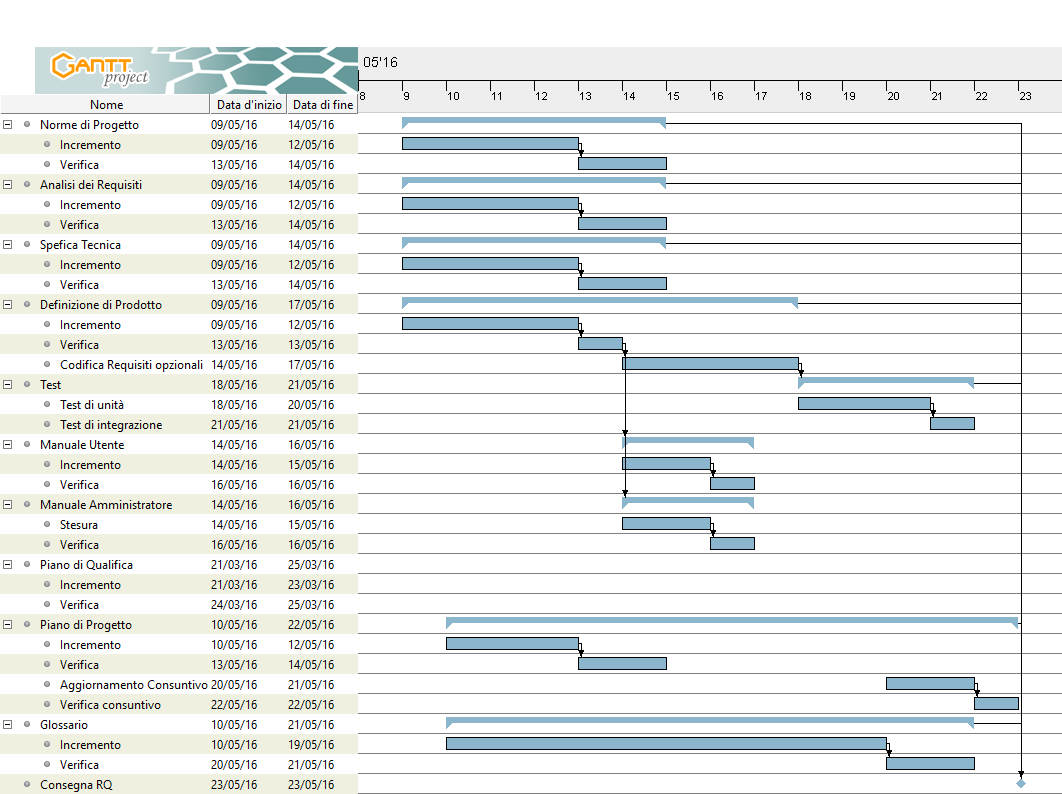
\includegraphics[width=\textwidth]{gantt_png/6-requisiti_facoltativi}
				\caption{Gantt - Fase PDROP}
				\label{fig:Gantt - Fase PDROP}
			\end{figure}
			

	\subsection{Fase V: Validazione}
		\textbf{Periodo: dal 2016-05-24 al 2015-06-17}
		
		Questa fase comincia con la consegna della Revisione di Qualifica e termina con la scadenza della consegna per la RA.

		\begin{itemize}
				\item Incremento e Verifica: se necessario verranno effettuati aggiornamenti ai vari documenti scritti;

				\item Validazione: viene verificato, attraverso tracciamento, di aver soddisfatto i requisiti presenti nel documento \textit{“Analisi dei Requisiti v1.00”};

				\item Esecuzione test: verranno eseguiti i test di sistema previsti dal documento \textit{“Piano di Qualifica v7.00”};

				\item Correzione bug: i bug rilevati verranno risolti;

				\item Collaudo: viene eseguito e completamente collaudato il sistema creato.
		\end{itemize}
		
		\subsubsection{Diagramma di Gantt – V}
			\begin{figure}[!h]
				\centering
				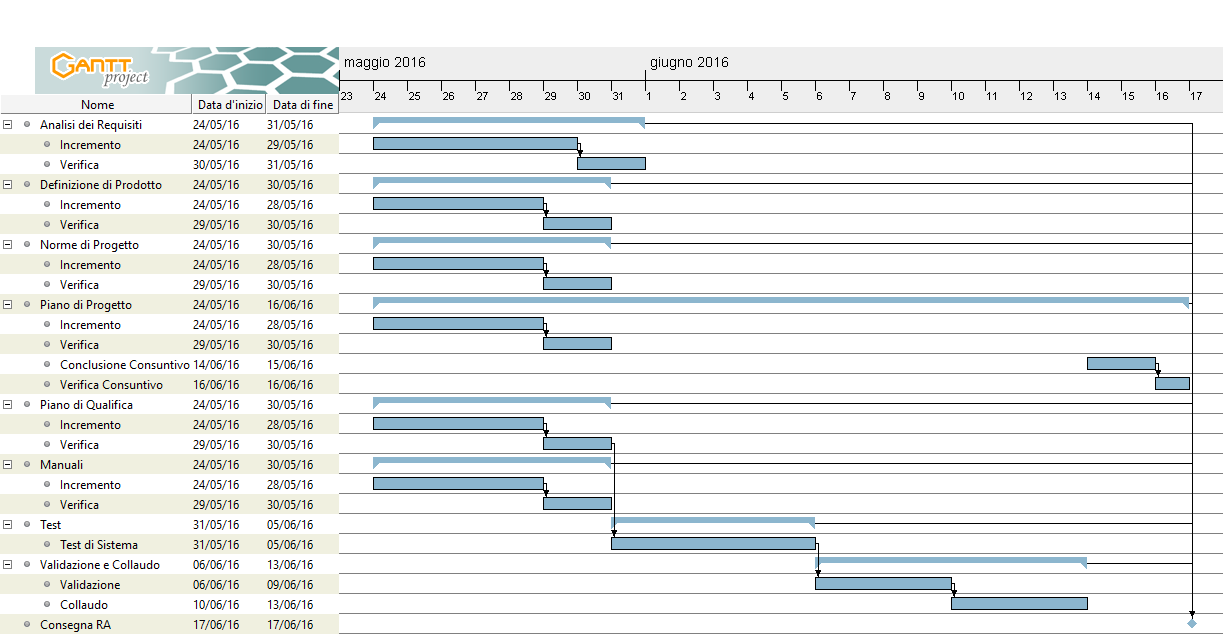
\includegraphics[width=\textwidth]{gantt_png/7-verifica}
				\caption{Gantt - Fase V}
				\label{fig:Gantt - Fase V}
			\end{figure}
			

\end{document}